% !TEX TS-program = pdflatex
% !TEX encoding = UTF-8 Unicode

% This is a simple template for a LaTeX document using the "article" class.
% See "book", "report", "letter" for other types of document.

\documentclass[a4paper,11pt]{article} % use larger type; default would be 10pt
\usepackage{listings}% la mierda para meter codigo

\usepackage[utf8]{inputenc} % set input encoding (not needed with XeLaTeX)
\usepackage{float} % para que las imagenes no se metan donde se les canta el orto

\setlength\parindent{24pt}

%%% Examples of Article customizations
% These packages are optional, depending whether you want the features they provide.
% See the LaTeX Companion or other references for full information.

%%% PAGE DIMENSIONS


\usepackage[legalpaper, landscape, margin=1in]{geometry}% to change the page dimensions
\geometry{a4paper} % or letterpaper (US) or a5paper or....
% \geometry{margin=2in} % for example, change the margins to 2 inches all round
% \geometry{landscape} % set up the page for landscape
%   read geometry.pdf for detailed page layout information

\usepackage{graphicx} % support the \includegraphics command and options
\usepackage{lmodern}% para evitar los warnings de fuentes

% \usepackage[parfill]{parskip} % Activate to begin paragraphs with an empty line rather than an indent

%%% PACKAGES
\usepackage[spanish]{babel} % para que el documento sea en argentino y de bokita el mas grande papá
\usepackage{booktabs} % for much better looking tables
\usepackage{array} % for better arrays (eg matrices) in maths
\usepackage{paralist} % very flexible & customisable lists (eg. enumerate/itemize, etc.)
\usepackage{enumitem} %Mierda de las listas para que se muestren indentadas
\usepackage{verbatim} % adds environment for commenting out blocks of text & for better verbatim
\usepackage{subfig} % make it possible to include more than one captioned figure/table in a single float
% These packages are all incorporated in the memoir class to one degree or another...

%%% HEADERS & FOOTERS
\usepackage{fancyhdr} % This should be set AFTER setting up the page geometry
\pagestyle{fancy} % options: empty , plain , fancy
\renewcommand{\headrulewidth}{0pt} % customise the layout...
\lhead{}\chead{}\rhead{}
\lfoot{}\cfoot{\thepage}\rfoot{}

%%% SECTION TITLE APPEARANCE
\usepackage{sectsty}
\allsectionsfont{\sffamily\mdseries\upshape} % (See the fntguide.pdf for font help)
% (This matches ConTeXt defaults)

%%% ToC (table of contents) APPEARANCE
\usepackage[nottoc,notlof,notlot]{tocbibind} % Put the bibliography in the ToC
\usepackage[titles,subfigure]{tocloft} % Alter the style of the Table of Contents
\renewcommand{\cftsecfont}{\rmfamily\mdseries\upshape}
\renewcommand{\cftsecpagefont}{\rmfamily\mdseries\upshape} % No bold!

%%% END Article customizations

%%% The "real" document content comes below...

\title{Práctica/Laboratorio de Capa de Enlace}
\author{Amoroso, Lihuel Pablo 13497/2; Gasquez, Federico Ramón 13598/6}
\date{Grupo A} % Activate to display a given date or no date (if empty),
         % otherwise the current date is printed

\begin{document}
\maketitle

\begin{figure}[htbp]
    \centering
    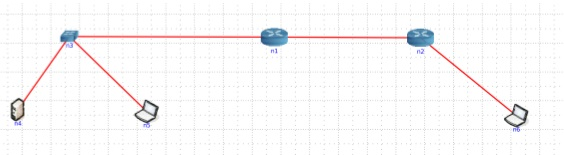
\includegraphics[]{imgs/topologia.jpg}
    \caption{Topología}
    \label{fig:topologia}
\end{figure}

\section{Genere la topología de la figura \ref{fig:topologia}, asigne direcciones IP y arme el ruteo para que todos sean “visibles” por IP.}

\subsection{Realice el comando ping(echo request) de n6 a n5 y capture el tráfico. Muestre encabezados Ethernet, y, de los contenidos, indique tipo de paquete, IP origen, IP destino cuando corresponda. Analice la diferencia entre las tramas IP y los mensajes ARP.}

\setlength{\leftskip}{0.5cm}N6(eth0)

\setlength{\leftskip}{1cm}ARP request

\indent\indent Encabezados Ethernet
\begin{itemize}
    \setlength{\itemindent}{80px}
    \item Src: 00:00:00\_aa:00:06 (00:00:00:aa:00:06)
    \item Dst: Broadcast (ff:ff:ff:ff:ff:ff)
    \item Type: ARP (0x0806)
\end{itemize}

\indent\indent Paquete ARP
\begin{itemize}
    \setlength{\itemindent}{80px}
    \item Sender IP address: 10.0.2.2 (10.0.2.2)
    \item Target IP address: 10.0.2.1 (10.0.2.1)
\end{itemize}

\setlength{\leftskip}{1cm}ARP reply

\indent\indent Encabezados Ethernet
\begin{itemize}
    \setlength{\itemindent}{80px}
    \item Src: 00:00:00\_aa:00:05 (00:00:00:aa:00:05)
    \item Dst: 00:00:00\_aa:00:06 (00:00:00:aa:00:06)
    \item Type: ARP (0x0806)
\end{itemize}

\indent\indent Paquete ARP
\begin{itemize}
    \setlength{\itemindent}{80px}
    \item Sender IP address: 10.0.2.1 (10.0.2.1)
    \item Target IP address: 10.0.2.2 (10.0.2.2)
\end{itemize}

\setlength{\leftskip}{1cm}ICMP request

\indent\indent Encabezados Ethernet
\begin{itemize}
    \setlength{\itemindent}{80px}
    \item Src: 00:00:00\_aa:00:06 (00:00:00:aa:00:06)
    \item Dst: 00:00:00\_aa:00:05 (00:00:00:aa:00:05)
    \item Type: IP (0x0800)
\end{itemize}

\indent\indent Paquete IP
\begin{itemize}
    \setlength{\itemindent}{80px}
    \item Source: 10.0.2.2 (10.0.2.2)
    \item Destination: 10.0.0.3 (10.0.0.3)
\end{itemize}

\setlength{\leftskip}{1cm}ICMP reply

\indent\indent Encabezados Ethernet
\begin{itemize}
    \setlength{\itemindent}{80px}
    \item Src: 00:00:00\_aa:00:05 (00:00:00:aa:00:05)
    \item Dst: 00:00:00\_aa:00:06 (00:00:00:aa:00:06)
    \item Type: IP (0x0800)
\end{itemize}

\indent\indent Paquete IP
\begin{itemize}
    \setlength{\itemindent}{80px}
    \item Source: 10.0.0.3 (10.0.0.3)
    \item Destination: 10.0.2.2 (10.0.2.2)
\end{itemize}

\setlength{\leftskip}{0.5cm}N2(eth0)\par
\setlength{\leftskip}{1cm}ARP request\par
\indent\indent Encabezados Ethernet
\begin{itemize}
    \setlength{\itemindent}{80px}
    \item Src: 00:00:00\_aa:00:04 (00:00:00:aa:00:04)
    \item Dst: 00:00:00\_aa:00:03 (00:00:00:aa:00:03)
    \item Type: ARP (0x0806)
\end{itemize}

\indent\indent Paquete ARP
\begin{itemize}
    \setlength{\itemindent}{80px}
    \item Sender IP address: 10.0.1.2 (10.0.1.2)
    \item Target IP address: 10.0.1.1 (10.0.1.1)
\end{itemize}

\setlength{\leftskip}{1cm}ARP reply\par
\indent\indent Encabezados Ethernet
\begin{itemize}
    \setlength{\itemindent}{80px}
    \item Src: 00:00:00\_aa:00:03 (00:00:00:aa:00:03)
    \item Dst: 00:00:00\_aa:00:04 (00:00:00:aa:00:04)
    \item Type: ARP (0x0806)
\end{itemize}

\indent\indent Paquete ARP
\begin{itemize}
    \setlength{\itemindent}{80px}
    \item Sender IP address: 10.0.1.1 (10.0.1.1)
    \item Target IP address: 10.0.1.2 (10.0.1.2)
\end{itemize}

\setlength{\leftskip}{1cm}ICMP request

\indent\indent Encabezados Ethernet
\begin{itemize}
    \setlength{\itemindent}{80px}
    \item Src: 00:00:00\_aa:00:04 (00:00:00:aa:00:04)
    \item Dst: 00:00:00\_aa:00:03 (00:00:00:aa:00:03)
    \item Type: IP (0x0800)
\end{itemize}

\indent\indent Paquete IP
\begin{itemize}
    \setlength{\itemindent}{80px}
    \item Source: 10.0.2.2 (10.0.2.2)
    \item Destination: 10.0.0.3 (10.0.0.3)
\end{itemize}

\setlength{\leftskip}{1cm}ICMP reply

\indent\indent Encabezados Ethernet
\begin{itemize}
    \setlength{\itemindent}{80px}
    \item Dst: 00:00:00\_aa:00:03 (00:00:00:aa:00:03)
    \item Src: 00:00:00\_aa:00:04 (00:00:00:aa:00:04)
    \item Type: IP (0x0800)
\end{itemize}

\indent\indent Paquete IP
\begin{itemize}
    \setlength{\itemindent}{80px}
    \item Source: 10.0.0.3 (10.0.0.3)
    \item Destination: 10.0.2.2 (10.0.2.2)
\end{itemize}

\setlength{\leftskip}{0.5cm}N1(eth0)

\setlength{\leftskip}{1cm}ARP request\par
\indent\indent Encabezados Ethernet
\begin{itemize}
    \setlength{\itemindent}{80px}
    \item Src: 00:00:00\_aa:00:02 (00:00:00:aa:00:02)
    \item Dst: Broadcast (ff:ff:ff:ff:ff:ff)
    \item Type: ARP (0x0806)
\end{itemize}

\indent\indent Paquete ARP
\begin{itemize}
    \setlength{\itemindent}{80px}
    \item Sender IP address: 10.0.0.1 (10.0.0.1)
    \item Target IP address: 10.0.0.3 (10.0.0.3)
\end{itemize}

\setlength{\leftskip}{1cm}ARP reply\par
\indent\indent Encabezados Ethernet
\begin{itemize}
    \setlength{\itemindent}{80px}
    \item Src: 00:00:00\_aa:00:01 (00:00:00:aa:00:01)
    \item Dst: 00:00:00\_aa:00:02 (00:00:00:aa:00:02))
    \item Type: ARP (0x0806)
\end{itemize}

\indent\indent Paquete ARP
\begin{itemize}
    \setlength{\itemindent}{80px}
    \item Sender IP address: 10.0.0.3 (10.0.0.3)
    \item Target IP address: 10.0.0.1 (10.0.0.1)
\end{itemize}

\setlength{\leftskip}{1cm}ICMP request

\indent\indent Encabezados Ethernet
\begin{itemize}
    \setlength{\itemindent}{80px}
    \item Src: 00:00:00\_aa:00:02 (00:00:00:aa:00:02)
    \item Dst: 00:00:00\_aa:00:01 (00:00:00:aa:00:01)
    \item Type: IP (0x0800)
\end{itemize}

\indent\indent Paquete IP
\begin{itemize}
    \setlength{\itemindent}{80px}
    \item Source: 10.0.2.2 (10.0.2.2)
    \item Destination: 10.0.0.3 (10.0.0.3)
\end{itemize}

\setlength{\leftskip}{1cm}ICMP reply

\indent\indent Encabezados Ethernet
\begin{itemize}
    \setlength{\itemindent}{80px}
    \item Src: 00:00:00\_aa:00:01 (00:00:00:aa:00:01)
    \item Dst: 00:00:00\_aa:00:02 (00:00:00:aa:00:02)
    \item Type: IP (0x0800)
\end{itemize}

\indent\indent Paquete IP
\begin{itemize}
    \setlength{\itemindent}{80px}
    \item Source: 10.0.0.3 (10.0.0.3)
    \item Destination: 10.0.2.2 (10.0.2.2)
\end{itemize}

\setlength{\leftskip}{0.5cm}N5(eth0)

\setlength{\leftskip}{1cm}ARP request\par
\indent\indent Encabezados Ethernet
\begin{itemize}
    \setlength{\itemindent}{80px}
    \item Src: 00:00:00\_aa:00:02 (00:00:00:aa:00:02)
    \item Dst: Broadcast (ff:ff:ff:ff:ff:ff)
    \item Type: ARP (0x0806)
\end{itemize}

\indent\indent Paquete ARP
\begin{itemize}
    \setlength{\itemindent}{80px}
    \item Sender IP address: 10.0.0.1 (10.0.0.1)
    \item Target IP address: 10.0.0.3 (10.0.0.3)
\end{itemize}

\setlength{\leftskip}{1cm}ARP reply\par
\indent\indent Encabezados Ethernet
\begin{itemize}
    \setlength{\itemindent}{80px}
    \item Src: 00:00:00\_aa:00:01 (00:00:00:aa:00:01)
    \item Dst: 00:00:00\_aa:00:02 (00:00:00:aa:00:02))
    \item Type: ARP (0x0806)
\end{itemize}

\indent\indent Paquete ARP
\begin{itemize}
    \setlength{\itemindent}{80px}
    \item Sender IP address: 10.0.0.3 (10.0.0.3)
    \item Target IP address: 10.0.0.1 (10.0.0.1)
\end{itemize}

\setlength{\leftskip}{1cm}ICMP request

\indent\indent Encabezados Ethernet
\begin{itemize}
    \setlength{\itemindent}{80px}
    \item Src: 00:00:00\_aa:00:02 (00:00:00:aa:00:02)
    \item Dst: 00:00:00\_aa:00:01 (00:00:00:aa:00:01)
    \item Type: IP (0x0800)
\end{itemize}

\indent\indent Paquete IP
\begin{itemize}
    \setlength{\itemindent}{80px}
    \item Source: 10.0.2.2 (10.0.2.2)
    \item Destination: 10.0.0.3 (10.0.0.3)
\end{itemize}

\setlength{\leftskip}{1cm}ICMP reply

\indent\indent Encabezados Ethernet
\begin{itemize}
    \setlength{\itemindent}{80px}
    \item Src: 00:00:00\_aa:00:01 (00:00:00:aa:00:01)
    \item Dst: 00:00:00\_aa:00:02 (00:00:00:aa:00:02)
    \item Type: IP (0x0800)
\end{itemize}

\indent\indent Paquete IP
\begin{itemize}
    \setlength{\itemindent}{80px}
    \item Source: 10.0.0.3 (10.0.0.3)
    \item Destination: 10.0.2.2 (10.0.2.2)
\end{itemize}

\paragraph{\textbf{Diferencia entre paquete IP y ARP}: la diferencia está en la capa y, por lo tanto, en qué dato se modifica. El paquete IP pertenece a una capa más alta que ARP y la IP destino y fuente no se modifican en todo el trayecto(incluso sería un problema si se modificaran, puesto que no se podría continuar); sin embargo, la IP emisora y receptora en los paquetes ARP en cada interfaz se va modificando conforme necesita encontrar la siguiente para poder continuar y que se lleve a cabo el PING.}

\subsection{Con la captura anterior, analice los mensajes ARP involucrados en el ruteo.}

    Analizando los mensajes anteriores ARP entre las diferentes interfaces, se puede observar que ARP funciona de la siguiente manera:

    \begin{enumerate}[leftmargin=2cm]
        \item Cuando una interfaz A quiere comunicarse con B envía un ARP request por broadcast, indicando que se busca la MAC de quien tenga la IP de B y que quien la tenga responda a A.
        \item El ARP request se distribuye por todo el dominio de broadcast y, si alguien tiene la IP buscada, es ese quién contesta con una ARP reply.
        \item Quien conteste el ARP request con un ARP reply sabe exactamente a quién contestarle: la información viene ya en el paquete.
        \item Cuando B recibe el ARP request y contesta, éste indica que la IP buscada se encuentra en tal dirección de MAC.
        \item Cuando A recibe el ARP reply de B, guarda la IP de B asociada a la MAC recibida. De esta manera es que A podrá comunicarse con B. Cada entrada tiene un TTL asociado, por lo que será necesario repetir este proceso periódicamente. Eventualmente, B podría guardarse también la MAC de A en su tabla ARP para futuras comunicaciones.
    \end{enumerate}

\subsection{En n1 agregue una entrada estática en la tabla de ARP con la IP de n4 y la MAC de n5. Limpie las tablas de ARP y vuelva a hacer el ping de n6 a n5. Capture en simultáneo el tráfico en n4 y n5.}

    Lo que hicimos fue agregar una tabla estatica en n1 con la IP de n4 y MAC de n5. Usamos el comando que está abajo. Luego realizamos el ping de n6 a n5. Mientras el ping se llevaba a cabo, se adjunta lo que recolectó el TCPdump.

    \begin{figure}[htbp]
        \centering
        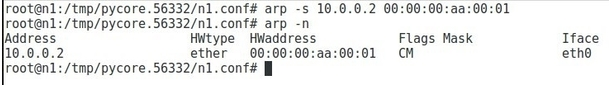
\includegraphics[]{imgs/comando_arp.png}
        \caption{Comando ARP utilizado y tabla}
        \label{fig:comando_arp}
    \end{figure}

    \begin{figure}[htbp]
        \centering
        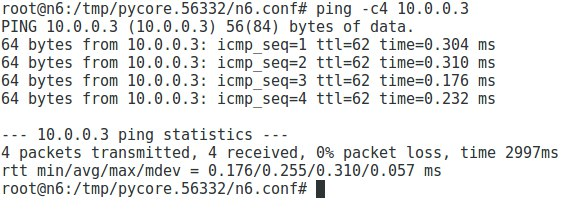
\includegraphics[]{imgs/ping_n6_n5.jpg}
        \caption{Ping de n6 a n5}
        \label{fig:ping_n6_n5}
    \end{figure}

    \begin{figure}[htbp]
        \centering
        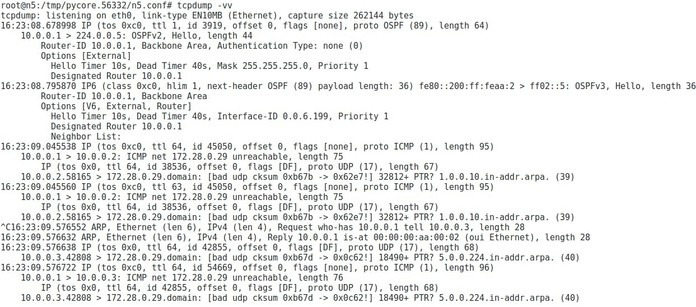
\includegraphics[]{imgs/tcpdump_n4.png}
        \caption{TCPdump de n4}
        \label{fig:tcpdump_n4}
    \end{figure}

    \begin{figure}[htbp]
        \centering
        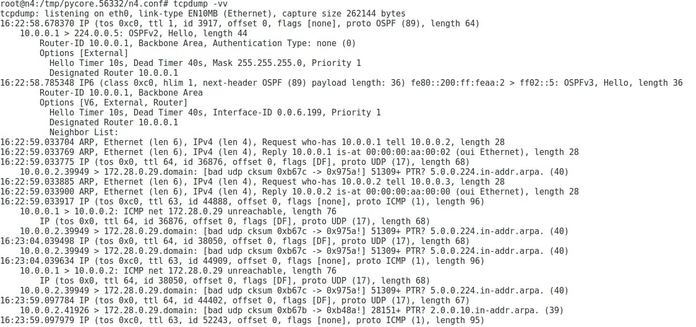
\includegraphics[]{imgs/tcpdump_n5.png}
        \caption{TCPdump de n5}
        \label{fig:tcpdump_n5}
    \end{figure}

\end{document}